% TeX eps-loader file generated by McmcDiagnostics.m (Dynare).
% 02-Oct-2019 00:52:21
 
\begin{figure}[H]
\psfrag{RA (m3)}[1][][0.5][0]{$ {r_{A}} $}
\psfrag{PA (Interval)}[1][][0.5][0]{$ {\pi^{(A)}} $}
\psfrag{PA (m2)}[1][][0.5][0]{$ {\pi^{(A)}} $}
\psfrag{PA (m3)}[1][][0.5][0]{$ {\pi^{(A)}} $}
\psfrag{GAMQ (Interval)}[1][][0.5][0]{$ {\gamma^{(Q)}} $}
\psfrag{GAMQ (m2)}[1][][0.5][0]{$ {\gamma^{(Q)}} $}
\psfrag{GAMQ (m3)}[1][][0.5][0]{$ {\gamma^{(Q)}} $}
\centering 
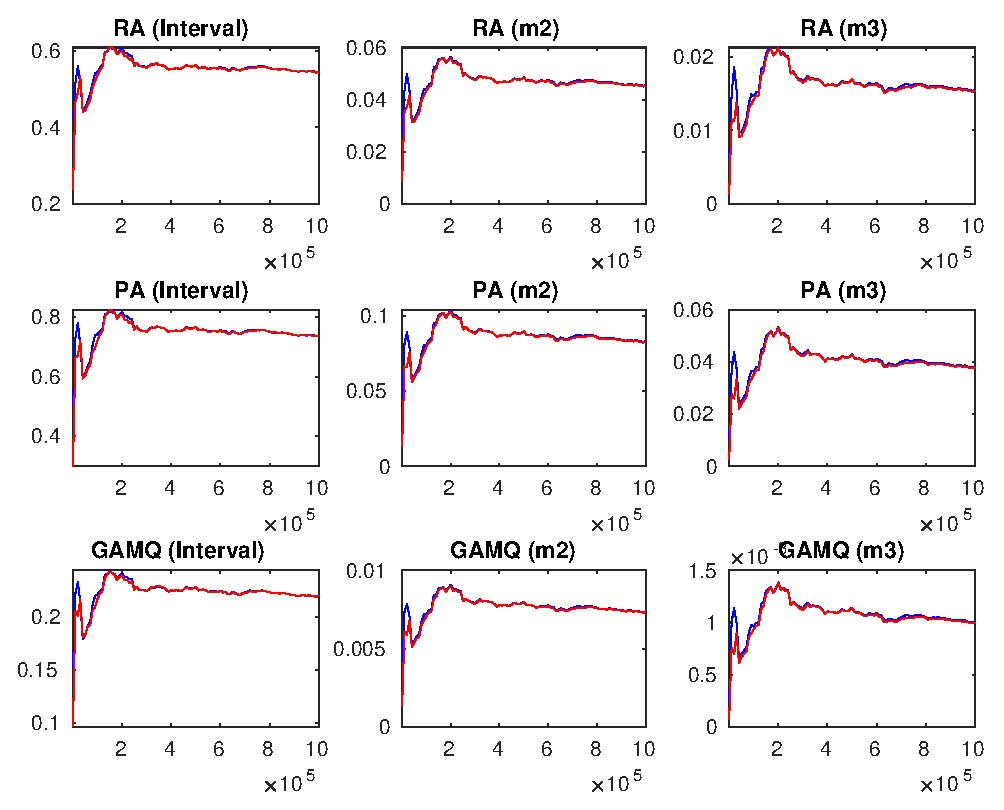
\includegraphics[width=0.80\textwidth]{AnSchoModTheBuilder/Output/AnSchoModTheBuilder_udiag1}
\caption{Univariate convergence diagnostics for the Metropolis-Hastings.
The first, second and third columns are respectively the criteria based on
the eighty percent interval, the second and third moments.}\label{Fig:UnivariateDiagnostics:1}
\end{figure}

\begin{figure}[H]
\psfrag{TAU (m3)}[1][][0.5][0]{$ {\tau} $}
\psfrag{NU (Interval)}[1][][0.5][0]{$ {\nu} $}
\psfrag{NU (m2)}[1][][0.5][0]{$ {\nu} $}
\psfrag{NU (m3)}[1][][0.5][0]{$ {\nu} $}
\psfrag{PSIP (Interval)}[1][][0.5][0]{$ {\psi_\pi} $}
\psfrag{PSIP (m2)}[1][][0.5][0]{$ {\psi_\pi} $}
\psfrag{PSIP (m3)}[1][][0.5][0]{$ {\psi_\pi} $}
\centering 
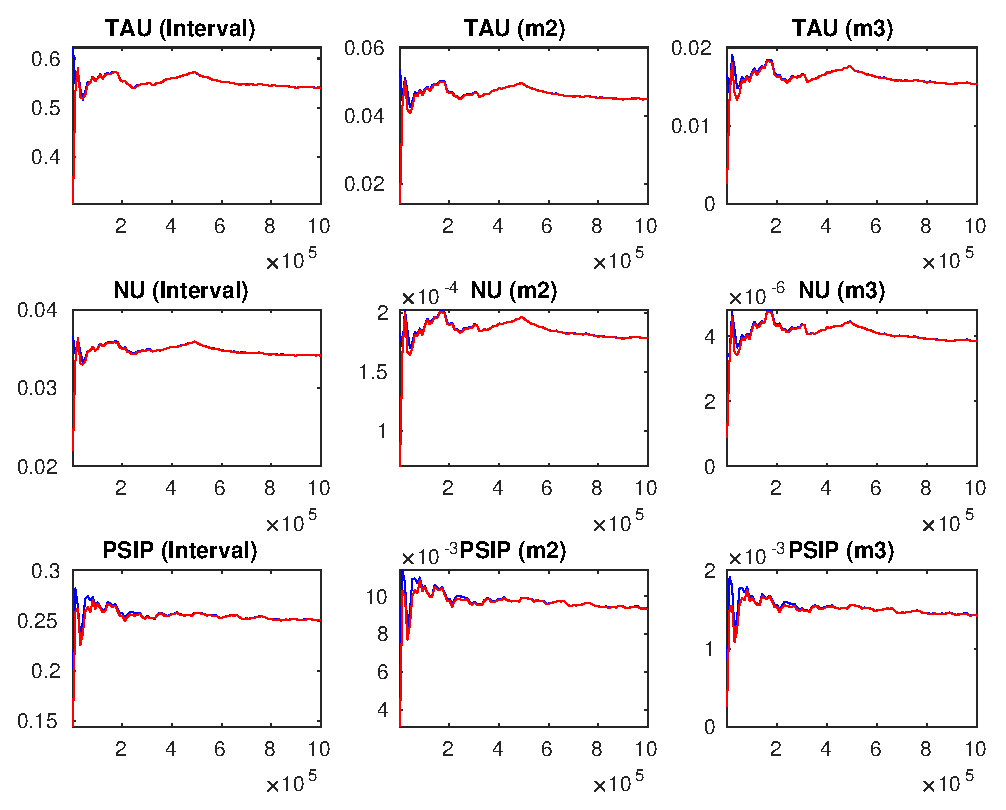
\includegraphics[width=0.80\textwidth]{AnSchoModTheBuilder/Output/AnSchoModTheBuilder_udiag2}
\caption{Univariate convergence diagnostics for the Metropolis-Hastings.
The first, second and third columns are respectively the criteria based on
the eighty percent interval, the second and third moments.}\label{Fig:UnivariateDiagnostics:2}
\end{figure}

\begin{figure}[H]
\psfrag{PSIY (m3)}[1][][0.5][0]{$ {\psi_y} $}
\psfrag{RHOR (Interval)}[1][][0.5][0]{$ {\rho_R} $}
\psfrag{RHOR (m2)}[1][][0.5][0]{$ {\rho_R} $}
\psfrag{RHOR (m3)}[1][][0.5][0]{$ {\rho_R} $}
\psfrag{RHOG (Interval)}[1][][0.5][0]{$ {\rho_{g}} $}
\psfrag{RHOG (m2)}[1][][0.5][0]{$ {\rho_{g}} $}
\psfrag{RHOG (m3)}[1][][0.5][0]{$ {\rho_{g}} $}
\centering 
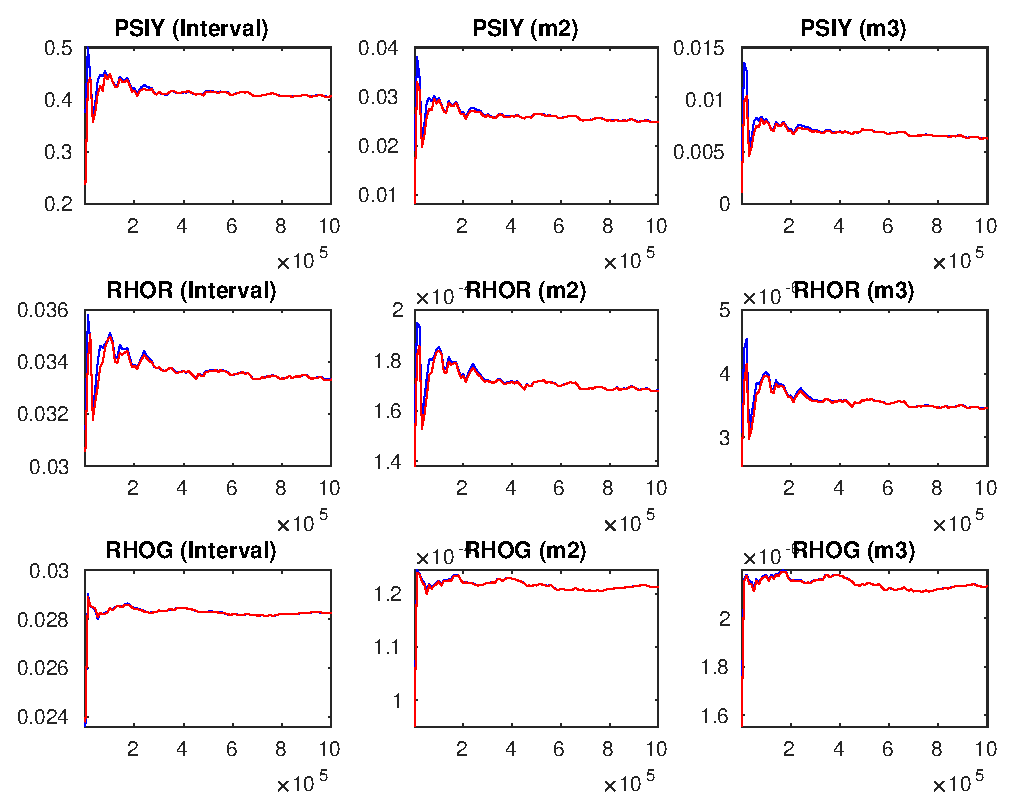
\includegraphics[width=0.80\textwidth]{AnSchoModTheBuilder/Output/AnSchoModTheBuilder_udiag3}
\caption{Univariate convergence diagnostics for the Metropolis-Hastings.
The first, second and third columns are respectively the criteria based on
the eighty percent interval, the second and third moments.}\label{Fig:UnivariateDiagnostics:3}
\end{figure}

\begin{figure}[H]
\psfrag{RHOZ (m3)}[1][][0.5][0]{$ {\rho_z} $}
\psfrag{SIGR (Interval)}[1][][0.5][0]{$ {\sigma_R} $}
\psfrag{SIGR (m2)}[1][][0.5][0]{$ {\sigma_R} $}
\psfrag{SIGR (m3)}[1][][0.5][0]{$ {\sigma_R} $}
\psfrag{SIGG (Interval)}[1][][0.5][0]{$ {\sigma_{g}} $}
\psfrag{SIGG (m2)}[1][][0.5][0]{$ {\sigma_{g}} $}
\psfrag{SIGG (m3)}[1][][0.5][0]{$ {\sigma_{g}} $}
\centering 
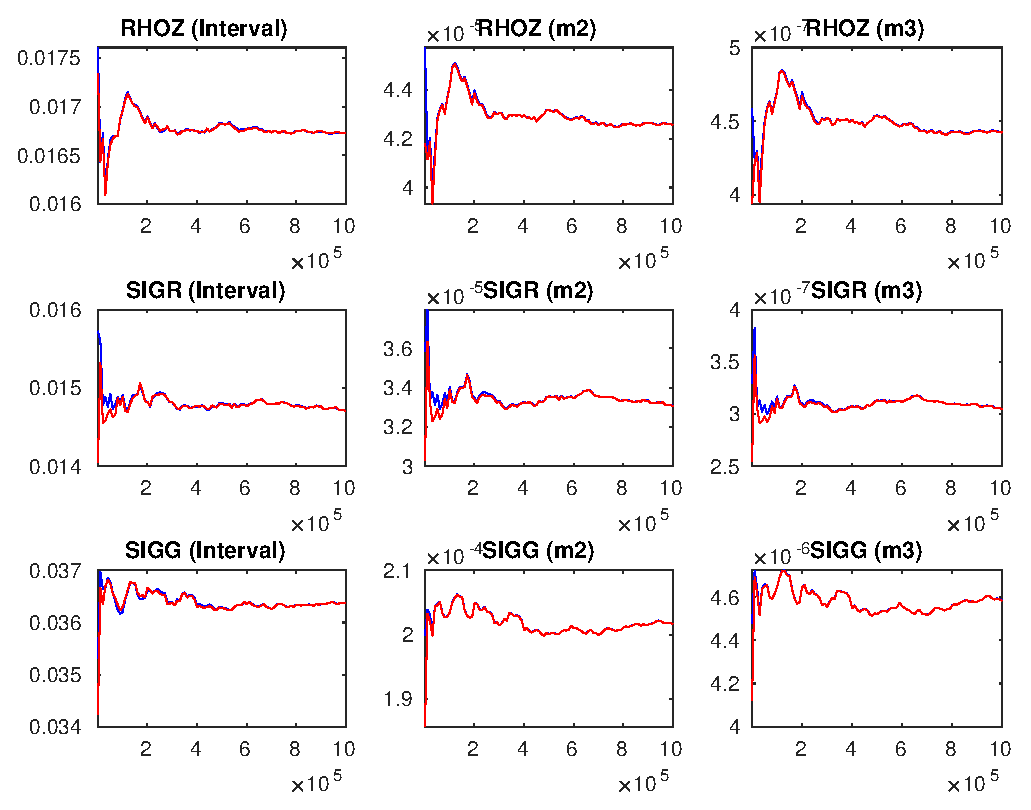
\includegraphics[width=0.80\textwidth]{AnSchoModTheBuilder/Output/AnSchoModTheBuilder_udiag4}
\caption{Univariate convergence diagnostics for the Metropolis-Hastings.
The first, second and third columns are respectively the criteria based on
the eighty percent interval, the second and third moments.}\label{Fig:UnivariateDiagnostics:4}
\end{figure}

\begin{figure}[H]
\psfrag{SIGZ (m3)}[1][][0.5][0]{$ {\sigma_z} $}
\centering 
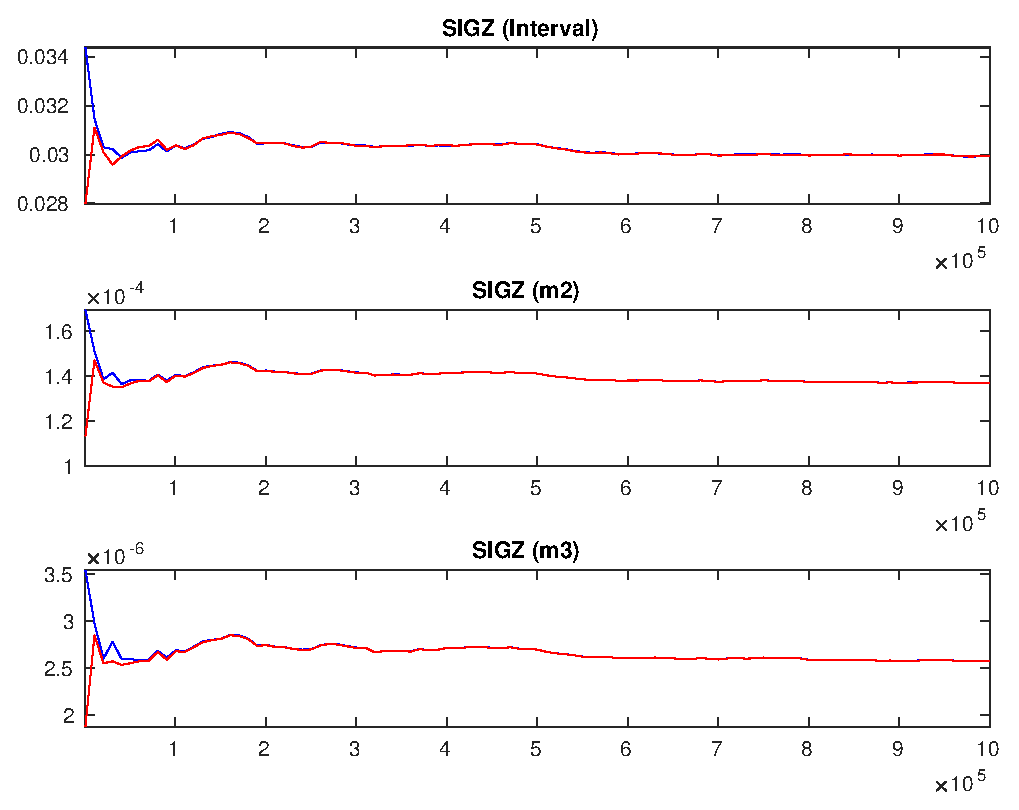
\includegraphics[width=0.80\textwidth]{AnSchoModTheBuilder/Output/AnSchoModTheBuilder_udiag5}
\caption{Univariate convergence diagnostics for the Metropolis-Hastings.
The first, second and third rows are respectively the criteria based on
the eighty percent interval, the second and third moments.}\label{Fig:UnivariateDiagnostics:5}
\end{figure}

